\chapter{Datensatz und Preprocessing}
\label{chap:dapre}
\pagebreak
\begin{table}[]
\subsection{Der Datensatz}
\centering
%\begin{tabular}{l r}
\begin{tabular*}{\textwidth}{c @{\extracolsep{\fill}} cc}
\toprule
\textbf{Merkmal} & \textbf{Beschreibung} \\
\midrule
 customernumber & individuelle Kundennummer\\
 \hline
 date & Datum der ersten Bestellung\\
 \hline
 salutation & Anrede des Kunden bzw. Firmenkunde\\
 \hline
 title & Titel vorhanden oder nicht\\
 \hline
 domain & Domain des Email Providers\\
 \hline
 datecreated & Datum der Accounterstellung\\
 \hline
 newsletter & wurde der Newsletter abboniert\\
 \hline
 model & nicht spezifiziert (Werte: 1,2,3)\\
 \hline
 paymenttype & gewählter Zahlungstyp\\
 \hline
 deliverytype & Versandart\\
 \hline
 invoicepostcode & Rechnungsadresse\\
 \hline
 delivpostcode & Lieferadresse\\
 \hline
 voucher & wurde ein Gutschein eingelöst\\
 \hline
 advertising & Werbecode\\
 \hline
 case & Wert der bestellten Produkte\\
 \hline
 numberitems & Anzahl der bestellten Artikel\\
 \hline
 gift & wurde die Geschenkoption verwendet\\
 \hline
 entry & Zugang zum Shop durch einen Partner oder nicht\\
 \hline
 points & wurden Punkte eingelöst\\
 \hline
 shippingcosts & sind Versandkosten angefallen\\
 \hline
 deliverydatepromised & versprochenes Lieferdatum\\
 \hline
 deliverydatepromised & tatsächliches Lieferdatum\\
 \hline
 weight & Gewicht der Bestellung\\
 \hline
 remi & Anzahl zurückgesendeter Artikel\\
 \hline
 cancel & Anzahl stornierter Artikel\\
 \hline
 used & Anzahl gebrauchter Artikel\\
 \hline
 w0 & Anzahl bestellter gebundener Bücher\\
 \hline
 w1 & Anzahl bestellter Taschenbücher\\
 \hline
 w2 & Anzahl bestellter Schulbücher\\
 \hline
 w3 & Anzahl bestellter eBooks\\
 \hline
 w4 & Anzahl bestellter Hörbücher\\
 \hline
 w5 & Anzahl heruntergeladener Hörbücher\\
 \hline
 w6 & Anzahl bestellter Filme\\
 \hline
 w7 & Anzahl bestellter Musikartikel\\
 \hline
 w8 & Anzahl bestellter Hardwareartikel\\
 \hline
 w9 & Anzahl bestellter importierter Artikel\\
 \hline
 w10 & Anzahl sonstige bestellte Artikel\\
 \hline
 \textbf{target90} & Zielvariable: Folgebestellung innerhalb von 90 Tagen oder nicht\\
\bottomrule
\end{tabular*}
\label{table: Features}
\caption{Übersicht aller Merkmale}
\end{table}
\FloatBarrier
\pagebreak

\subsection{Die Zielvariable}

Die Zielvariable target90 gibt an, ob ein Kunde innerhalb von 90 Tagen erneut eine Bestellung beim Online-Händler getätigt hat oder nicht. Es handelt sich um eine nominalskalierte Variable, welche als Ganzzahl codiert worden ist. Das Klassenlabel ist in Trainings- und Testdatensatz für alle Einträge angegeben. Deswegen handelt es sich hierbei um überwachtes Lernen. Dadurch, dass ausschließlich zwei Ausprägungen möglich sind, bezeichnet man die Aufgabenstellung als binäre Klassifikation.\\

In Abbildung \ref{fig:classDist} ist die Verteilung der Zielvariable für Trainings- und Testdaten dargestellt. Es wird deutlich, dass in beiden Datensätzen eine ähnliche Verteilung vorliegt. Rund 80 \% der Einträge nehmen die Ausprägung 0 an. Das heißt, dass 80 \% der Kunden nach der Erstbestellung nicht innerhalb von 90 Tagen erneut bestellen. Dagegen sind 20 \% der Kunden als Wiederkäufer etikettiert. Diese Verteilung zeigt die Unbalanciertheit der beiden Klassen.\\

Die fehlende Gleichverteilung kann im Zuge der Modellbildung und Klassifikation zu falschen Ergebnissen führen. Das begründet sich darin, dass die meisten Algorithmen implizit eine Gleichverteilung der Klassen annehmen. Es gibt deutlich weniger Trainingsbeispiele, um die Eigenschaften der unterrepräsentierten Klasse zu erlernen. Das kann zu Klassifikatoren führen, welche lediglich die überrepräsentierte Klasse vorhersagen. Diese Beobachtung führt dazu, dass im späteren Verlauf des Modellbildungsprozesses Resampling-Strategien angewendet werden.

\begin{figure}[!htbp]
\begin{center}
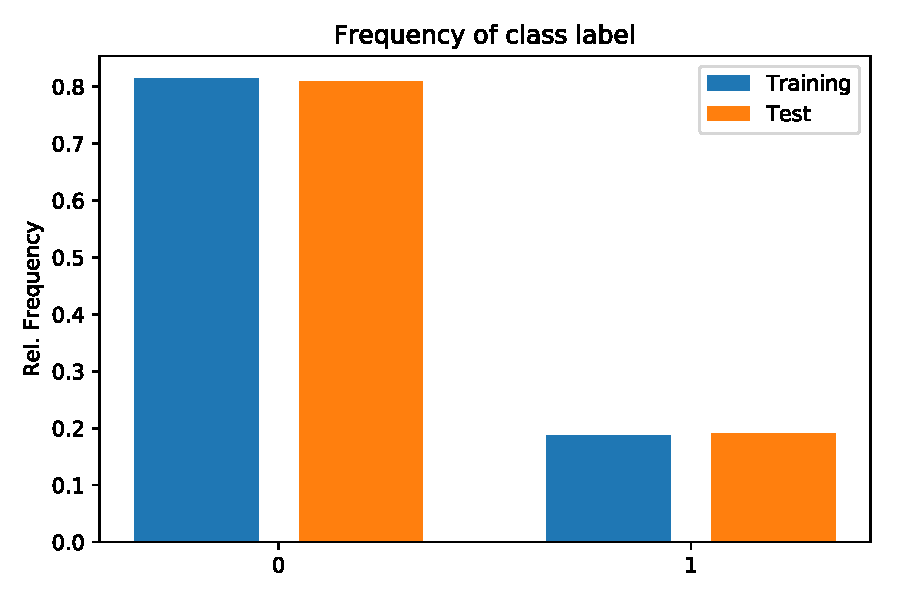
\includegraphics[scale=0.5]{pdf/distTrainTest.pdf}
\end{center}
\caption{Klassenverteilung in Trainings- und Testdaten}
\label{fig:classDist}
\end{figure}
\FloatBarrier
\pagebreak

\subsection{Feature Engingeering}
Ein wichtiger Schritt der Datenvorverarbeitung ist einerseits das Löschen irrelevanter Features. Andererseits wird beim Feature Engineering versucht neue, aussagekräftigere Merkmale aus den bestehenden zu erzeugen oder bestehende so zu bearbeiten, dass sie bestmöglich für den nachgeschalteten Klassifikationsalgorithmus geeignet sind. Im Folgenden werden die neu konstruierten Merkmale beschrieben:

\subsubsection{Konstruierte Attribute}

\textbf{accountdur:}\\


\textbf{books:}\\



\textbf{nobooks:}\\


\textbf{itemseff:}\\

Aus der Anzahl der bestellten Artikel, abzüglich der stornierten und zurückgegebenen Artikel, wird die Anzahl der tatsächlich gekauften Artikel erstellt (itemseff). Dieses Merkmal gibt an, wie viele Artikel effektiv durch den Kunden gekauft worden sind.

\subsubsection{Modifizierte Attribute}

\textbf{OneHotEncoding:}\\

Algorithmen des maschinellen Lernens können nicht unmittelbar mit kategorialen Merkmalen arbeiten. Damit trotzdem Modelle mit diesen Features trainiert werden können, müssen die Ausprägungen der Merkmale zunächst in einen ganzzahligen Wert codiert werden. Damit die Merkmale anschließend nicht als numerisches Merkmal interpretiert werden ist One Hot Encoding nötig.\\

Beim One Hot Encoding wird aus den codierten Merkmalen ein Binärer Vektor erstellt. Die Ausprägungen werden dadurch repräsentiert, dass nur die Spalte des Merkmals den Wert 1 annimmt und die anderen Spalten 0 werden. Besonders deutlich wird dies im Teil Modeling. Die dort trainierten Entscheidungsbäume (CART) nutzen nur binäre Splits. Die binären Splits treffen Entscheidungen anhand von „größer gleich oder kleiner gleich“ Beziehungen. Auf die nachfolgenden kategorialen Variablen wird deshalb One Hote Encoding angewendet, um richtige Ergebnisse zu gewährleisten.\\


\textbf{salutation:}\\

Die Anrede des Kunden nimmt drei Ausprägungen an. Ein Kunde wird als männlich, weiblich oder als Firmenkunde erfasst. Das Merkmal ist bereits im Datensatz als Ganzzahl repräsentiert. Aufgrund des nominalen Skalenniveaus und der Überschreitung von zwei Ausprägungen wird das Merkmal durch One Hot Encoding transformiert. 

\textbf{model:}\\

Die Bedeutung des Features model ist nicht genauer spezifiziert. Wir können dennoch nicht daraus schließen, dass das Merkmal unbedeutsam für die Klassifikationsgüte ist. Das Merkmal nimmt ebenfalls drei Ausprägungen an. Die Ausprägungen sind bereits als Ganzzahl codiert und deshalb ist nur noch die Vektorisierung des Merkmals durch One Hot Encoding nötig. Die Transformation erzeugt drei neue Spalten in unserer Merkmalsmatrix. Inwiefern das Merkmal tatsächlich Relevanz hat, wird bei einer Feature Selection im Evaluationsteil bewertet.\\

\textbf{paymenttype:}\\

Der Zahlungstyp besitzt die vier, bereits codierten Ausprägungen Zahlung auf Rechnung, Barzahlung, Zahlung mit dem bestehenden Account und per Kreditkarte. Das Merkmal wird ebenfalls in die Merkmalsmatrix aufgenommen und zuvor mit One Hot Encoding transformiert.

\subsubsection{Gelöschte Attribute}

\textbf{deliverydatereal und deliverydatepromised:}\\


\textbf{datecreated und date:}\\

Aus dem Datum der Accounteröffnung datecreated und dem Datum der Erstbestellung date wird das Merkmal accountdur konstruiert. Dieses gibt die Anzahl der Tage von der Accounteröffnung bis zur ersten Lieferung an. Das neue Merkmal hat zur Folge, dass die beiden genannte Merkmale gelöscht werden.\\

\textbf{customernumber:}\\

Die Kundennummer wird gelöscht, weil sie aufgrund ihrer Individualität keine Gruppierung bezüglich der beiden Klassen ermöglicht.\\

\textbf{invoicepostcode und delivpostcode:}

\textbf{domain:}\\

\textbf{points:}\\

Das nominalskalierte Merkmal points gibt an, ob bei der Bestellung Punkte eingelöst worden sind. In der Phase des Data Understandings hat sich gezeigt, dass dieses Merkmal ausschließlich den Wert 0 annimmt. Es wird deshalb aus der Merkmalsmatrix entfernt.\\

\textbf{title:} \\

\textbf{gift:}\\

\pagebreak

\subsection{Resampling}
\begin{figure}[!htbp]
\begin{center}
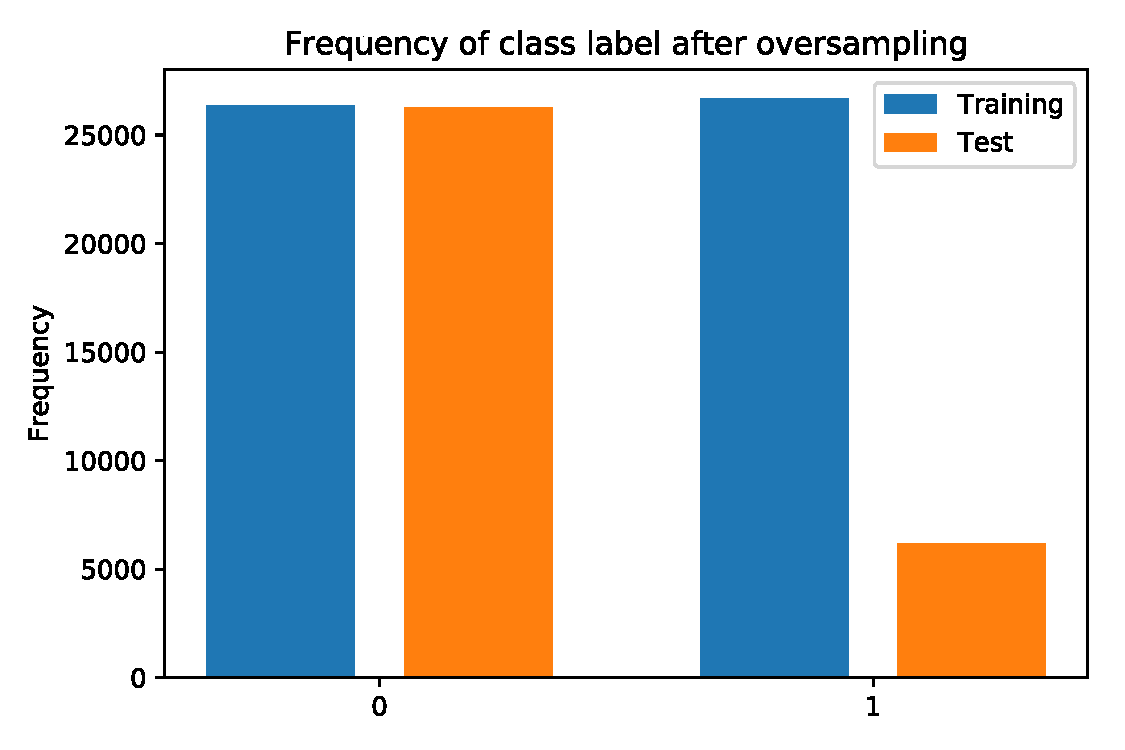
\includegraphics[scale=0.5]{pdf/oversampled.pdf}
\end{center}
\caption{Klassenverteilung nach Oversampling der Minderheitsklasse}
\label{fig:over}
\end{figure}
\FloatBarrier
\chapter{Modeling und Evaluation}
\section{Modeling}

\subsection{Entscheidungsbaum Klassifikator}
\label{sec:Tree}


\subsection{Random Forests}
\label{sec:RF}

 

\section{Evaluation}
\label{sec:eval}
\subsection{Das Evaluationskriterium}



\subsection{Backward Feature Elimination}

\FloatBarrier
\begin{figure}[!htbp]
\begin{center}
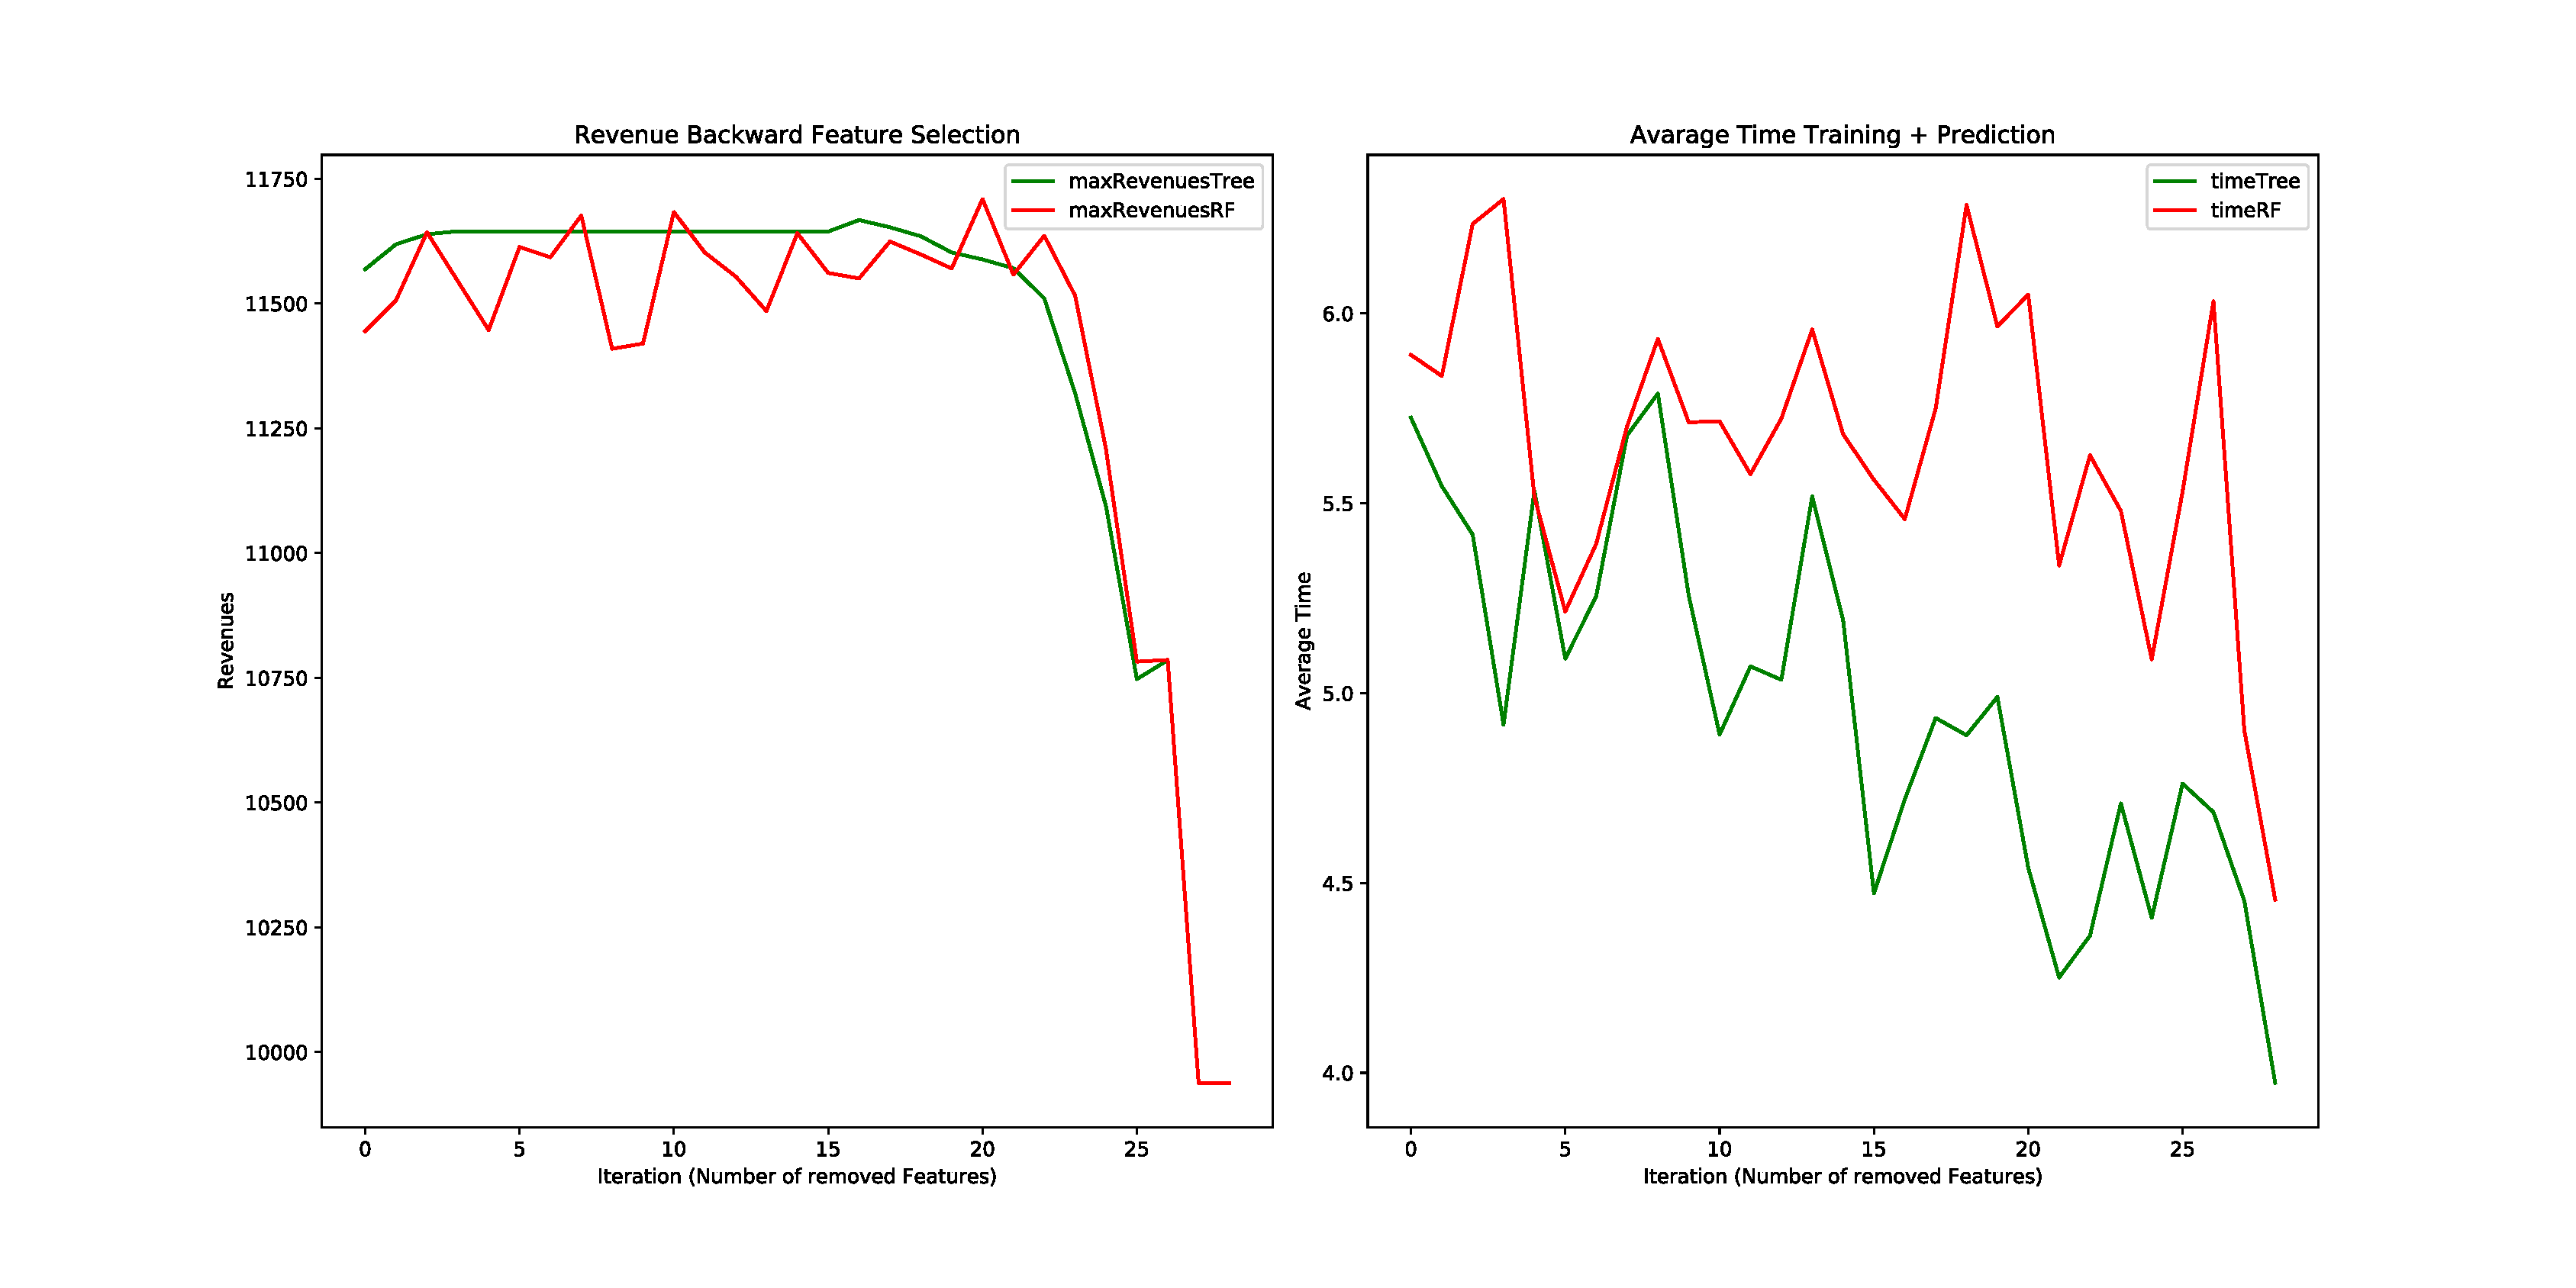
\includegraphics[scale=0.3]{pdf/backwardSpark.pdf}
\end{center}
\caption{Umsatz in Anbhängigkeit zur Anzahl der entfernten Merkmale}
\label{fig:backwardSpark}
\end{figure}
\FloatBarrier

\begin{table}[]
\centering
%\begin{tabular}{c c c c c c l}
\begin{tabular*}{\textwidth}{c @{\extracolsep{\fill}} lllllll}
\toprule
\textbf{i} & \textbf{Rev DT} & \textbf{t in sec} & \textbf{dropped DT} & \textbf{Rev RF} & \textbf{t in sec} &\textbf{dropped RF} \\
\midrule
1 & 11569.00 & 5.73 & shippingcosts & 11444.50 & 5.89 & numberitems \\
2 & 11619.00 & 5.55 & modelVec & 11507.00 & 5.84 & nobooks \\
3 & 11639.00 & 5.42 & salutationVec & 11643.00 & 6.24 & w8 \\
4 & 11645.00 & 4.92 & entry & 11545.00 & 6.30 & entry \\
5 & 11645.00 & 5.53 & case & 11447.00 & 5.52 & w3 \\
6 & 11645.00 & 5.09 & numberitems & 11613.50 & 5.22 & itemseff \\
7 & 11645.00 & 5.25 & gift & 11593.00 & 5.39 & w0 \\
8 & 11645.00 & 5.68 & w0 & 11676.50 & 5.70 & books \\
9 & 11645.00 & 5.79 & w2 & 11409.50 & 5.93 & w4 \\
10 & 11645.00 & 5.26 & w3 & 11420.00 & 5.71 & modelVec \\
11 & 11645.00 & 4.89 & w4 & 11683.50 & 5.72 & w2 \\
12 & 11645.00 & 5.07 & w6 & 11602.50 & 5.58 & gift \\
13 & 11645.00 & 5.04 & w8 & 11554.50 & 5.72 & accountdur \\
14 & 11645.00 & 5.52 & w9 & 11485.00 & 5.96 & cancel \\
15 & 11645.00 & 5.19 & nobooks & 11641.00 & 5.68 & w7 \\
16 & 11644.50 & 4.47 & books & 11561.50 & 5.56 & w5 \\
17 & 11667.50 & 4.72 & w7 & 11550.50 & 5.46 & w6 \\
18 & 11653.00 & 4.93 & w5 & 11624.50 & 5.75 & w10 \\
19 & 11635.00 & 4.89 & w10 & 11598.50 & 6.29 & w9 \\
20 & 11602.50 & 4.99 & cancel & 11570.50 & 5.97 & salutationVec \\
21 & 11588.50 & 4.54 & voucher & 11709.50 & 6.05 & shippingcosts \\
22 & 11571.00 & 4.25 & accountdur & 11558.00 & 5.34 & case \\
23 & 11510.50 & 4.36 & used & 11636.00 & 5.63 & voucher \\
24 & 11320.50 & 4.71 & itemseff & 11516.00 & 5.48 & used \\
25 & 11094.00 & 4.41 & weight & 11208.00 & 5.09 & weight \\
26 & 10747.50 & 4.76 & w1 & 10782.50 & 5.53 & paymenttypeVec \\
27 & 10785.50 & 4.69 & paymenttypeVec & 10786.00 & 6.03 & w1 \\
28 & 9938.50 & 4.45 & remi & 9938.50 & 4.90 & remi \\
29 & 9938.50 & 3.97 & newsletter & 9938.50 & 4.46 & newsletter \\
\bottomrule
\end{tabular*}
\caption{Ergebnisse Backward Feature Elimination}
\label{table: Backward}
\end{table}
\FloatBarrier
 
 

\FloatBarrier
\begin{figure}[!htbp]
\begin{center}
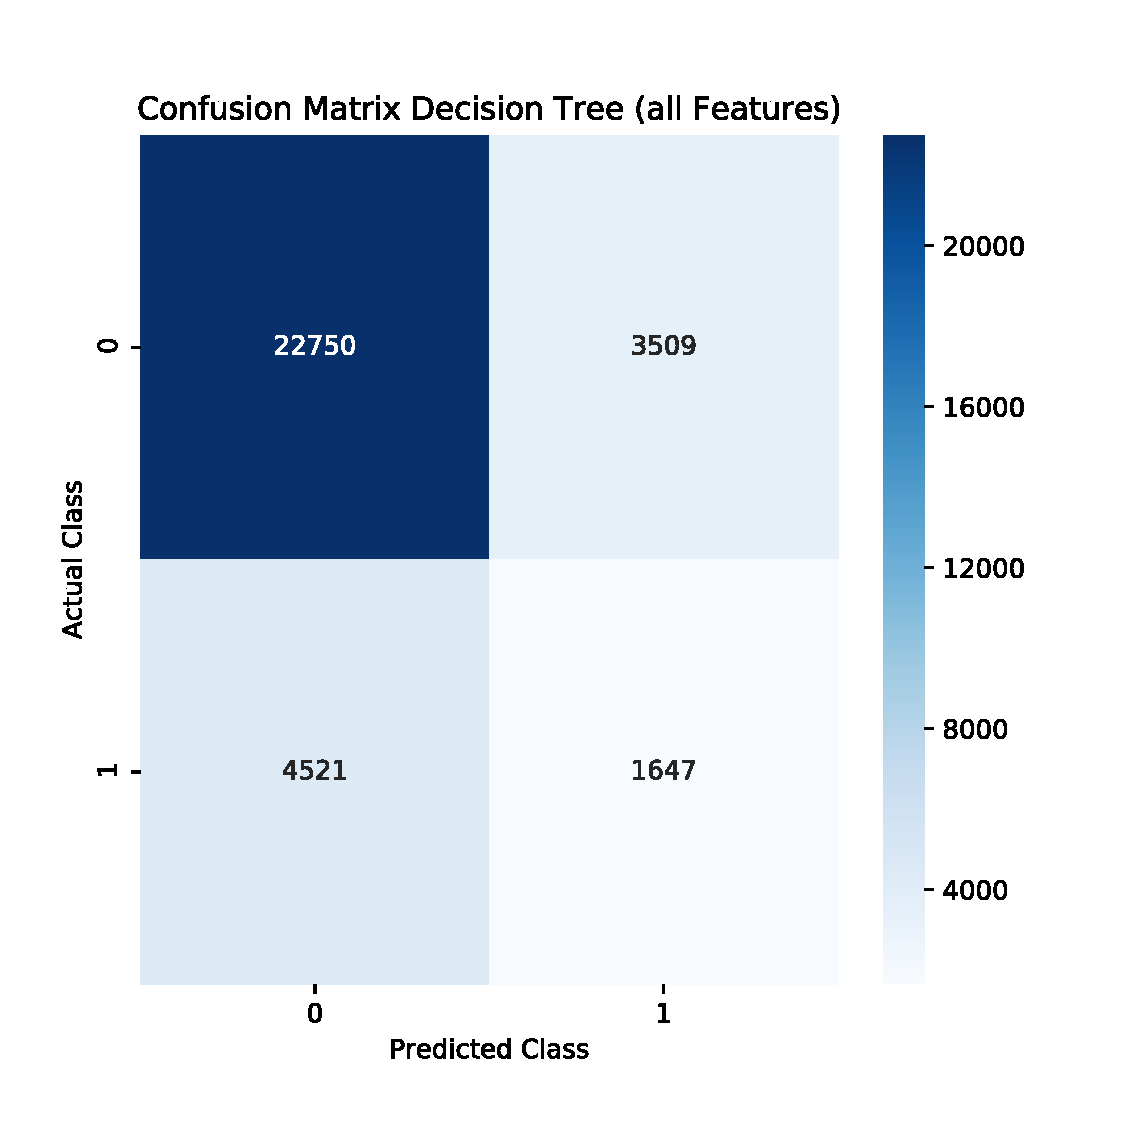
\includegraphics[scale=0.5]{pdf/confusion2.pdf}
\end{center}
\caption{Konfusionsmatrix Decision Tree mit allen Merkmalen}
\label{fig:confusionFinal}
\end{figure}
\FloatBarrier

\chapter{Zusammenfassung}






